\documentclass{article}
\usepackage{arxiv}

\usepackage[utf8]{inputenc}
\usepackage[english, russian]{babel}
\usepackage[T1]{fontenc}
\usepackage{url}
\usepackage{booktabs}
\usepackage{amsfonts}
\usepackage{nicefrac}
\usepackage{microtype}
\usepackage{lipsum}
\usepackage{graphicx}
\usepackage{svg}
\usepackage{natbib}
\usepackage{doi}
\usepackage{booktabs}
\usepackage{float}
\usepackage{mathtools}
\usepackage[russian]{babel}      % пакет русификации
\usepackage{amsmath}
\usepackage{tikz}                % для создания иллюстраций
\usepackage{pgfplots}            % для вывода графиков функций
\usepackage{geometry}		 % для настройки размера полей
\usepackage{hhline}
\usepackage{placeins}
\usepackage{indentfirst}         % для отступа в первом абзаце секции
\usepackage{multirow}            % для таблицы с результатами
\usepackage{svg}
\usepackage{makecell}
\usepackage{listings}
\usepackage{float}
\usepackage[unicode, colorlinks, linkcolor=Black]{hyperref}

\title{Мера сходства элементов штрихового представления рукописного текста на~основе Фурье-дескриптора}

\author{ Феоктистов Дмитрий Дмитриевич \\
	ВМК МГУ\\
	\texttt{feoktistovdd@my.msu.ru} \\
	%% examples of more authors
	\And
	Местецкий Леонид Моисеевич \\
	ВМК МГУ, НИУ ВШЭ\\
	\texttt{mestlm@yandex.ru} \\
}
\date{2023}

\renewcommand{\shorttitle}{Классификация дуктов для поиска ключевых слов в рукописном контексте}

%%% Add PDF metadata to help others organize their library
%%% Once the PDF is generated, you can check the metadata with
%%% $ pdfinfo template.pdf
\hypersetup{
pdftitle={Поиск ключевых слов в рукописном контексте},
pdfsubject={q-bio.NC, q-bio.QM},
pdfauthor={Феоктистов Д.Д., Местецкий Л.М.},
pdfkeywords={First keyword, Second keyword, More},
}

\begin{document}
\maketitle
\begin{abstract}
В работе изучается задача классификации элементов штрихового разложения рукописного текста. Для ее решения предлагается использовать векторизацию штрихов на основе преобразования Фурье, после чего использовать полученные вектора в метрических классификаторах. Полученный в ходе работы классификатор штрихов предлагается использовать как часть ранжирующего алгоритма для задачи поиска ключевых слов в рукописном контексте. Решение этой задачи может значительно упростить работу с архивными данными. В ходе экспериментов с изображениями панграмм показано, что для описания штриха достаточно малого количества коэффициентов (5-7 штук), а также, что предлагаемый подход является наилучшим по соотношению скорость/качество классификации. 
 % После чего строится алгоритм ранжирования слов, использующий информацию о классах штрихов запроса и слов контекста. Для демонстрации результатов работы используются изображения работ участников ''Тотального диктанта''.
\end{abstract}


\keywords{Преобразование Фурье \and Штриховая сегментация текста \and Обнаружение ключевых слов \and Компьютерное зрение}

\section{Введение}
\par Задача поиска ключевых слов в рукописном контексте является актуальной последние десятилетия в силу того, что полноценное распознавание рукописного текста не достигло той точности, при которой можно выполнять полноценное чтение документа и поиск в нем \citep{10.1007/978-3-031-36616-1_15, SOUIBGUI202243}. Одной из главной целей при решении задачи является достижение ее применимости для навигации в архивных документах \citep{10.1007/978-3-319-13695-0_74, 7333824}. 
\par Изначально задача поиска ключевых слов решалась для напечатанных документов, в которых используется курсивный шрифт \citep{627095}. Постепенно задача стала усложняться, и появились алгоритмы, выполняющие поиск в рукописных текстах \citep{1211511}, .
\par Существует несколько разновидностей рассматриваемой задачи. В первом варианте запрос задается в виде примера искомого слова в данном документе, такой подход позволяет обойти проблему разнообразия почерков \citep{7333824, 8378004}. Более общий подход предполагает, что запрос является строкой \citep{retsinas2021from}. Путей решения задачи также существует несколько. Первый предполагает использование глубоких нейронных сетей напрямую \citep{10.1007/978-3-031-41676-7_26, 10.1007/978-3-031-06555-2_26, Cascianelli2022}, второй -- использование нейронных сетей для построения векторных представлений слов для осуществления последующего поиска \citep{retsinas2021from, Krishnan2023, jemni2023stkeys}. Третий же стоит отдельно и предполагает использование признаков, полученных из изображения с помощью некоторых алгоритмов, с последующим их применением в алгоритмах машинного обучения. При этом может использоваться как и дискретное представление слов \citep{8270021, yousfi2021keyword, kundu2021hough}, так и непрерывные признаки, полученные из скелетных графов \citep{7333824, ameri2017keyword, stauffer2016graph}. Последний подход является актуальным и по сей день \citep{yousfi2021keyword, kundu2021hough, banerjee2022z}, так как есть экспериментально подтвержденная гипотеза о том, что увеличение количества параметров в нейронных сетях не приводит к улучшению результатов поиска \citep{rusakov2018expolring}. Наиболее актуальные алгоритмы используют комбинацию описанных подходов, применяя как и классические признаки, так и полученные с помощью обучения нейронной сети \citep{jemni2023stkeys, omayio2023word}.
\par Отдельно стоит выделить алгоритмы, выполняющие сопоставление запроса и слова с помощью различных метрик. Этот подход интересен тем, что метрики являются интерпретируемыми \citep{ameri2017keyword, stauffer2016graph}. При этом большинство метрик вычисляются долго, из-за чего требуется разработка специальных фильтров, позволяющих ускорять поиск \citep{stauffer2020filters}.
\par В данной работе предлагается новый метод решения задачи поиска ключевых слов в рукописном контексте, основанный на следующей гипотезе: все почерки являются вариацией некоторого эталонного. Действительно, уже несколько веков обучение письму производится с помощью прописей, в которых не меняются правила написания штрихов (дуктов), из которых строятся буквы \citep{austin2010}. Соответственно, если задать метрику близости на штрихах и произвести их классификацию \citep{pronina2023frechet, pazazia2023dtw}, то получится обоснованное представление слова в виде частично упорядоченного множества (порядок возникает из-за порядка появления штрихов). Имея описанное выше представление, можно производить поиск ключевых слов с помощью различных мер схожести множеств штрихов. Также описанная выше гипотеза позволяет решать задачу поиска ключевых слов в формулировке, в которой запрос передается в виде строки, которая преобразуется в изображение, написанное с помощью эталонного почерка \citep{retsinas2021from}. Насколько авторам известно, в подобной формулировке задача решалась в \citep{pronina2023frechet, pazazia2023dtw}, где для сравнения штрихов использовалось расстояние Фреше и DTW соответственно, но в этих работах рассматривался подход основанный на кластеризации, в то время как классификация способна дать больше информации. Таким образов в данной статье описаны:
\begin{enumerate}
\item Алгоритм выделения штрихов из изображения рукописного слова, основанный на построении скелета изображения.
\item Метрика для задачи классификации на пространстве дуктов, основанной на преобразовании Фурье ломанных, описывающих штрихи.
% \item Мера сходства слов, использующая для поиска релевантных слов, основанная на расстоянии Левенштейна между множествами классифицированных дуктов.
\end{enumerate}
Для демонстрации результатов работы полученного алгоритма используется изображение с несколькими панграммами: текстами, содержащими все буквы алфавита.
\section{Задача поиска ключевых слов в рукописном контексте}
Цель поиска ключевых слов состоит в том, чтобы извлечь изображения слов из заданной коллекции изображений документов и ранжировать их по релевантности определенному запросу. Запрос может быть либо уже найденным пользователем изображением слова (т.е. обрезанное изображение документа) (QbE), либо строкой, отвечающей слову, которое необходимо найти (QbS). Главным преимуществом второй постановки является отсутствие необходимости искать пользователю запрашиваемое слово самостоятельно, что сильно экономит время при работе с редкими словами, поэтому в данной работе рассматривается вариант QbS. Формализуем данную постановку. Пусть у нас есть множество строк $S$ и множество изображений слов $W$. Пусть $c(w)$ - строка, соответствующая изображению $w$. Тогда нам надо найти такое отображение $f: S \times W \rightarrow \mathbb{R}$, что:
$$argmin_w f(c(w_1), w) = w_1\;\;\;\forall w_1 \in W$$
В задаче поиска ключевых слов общепринятой метрикой является  $mean\; average\; precision$:
$$MAP = \frac{1}{|Q|}\sum_{q \in Q}AP(q)$$
Где $AP(q)$ -- площадь под кривой $precision-recall$ кривой для запроса $q$.\\
\section{Задача метрической классификации штрихов}
Математической моделью штриха является ломаная, которая может быть как замкнута, так и являться цепью. Существенным ограничением является отсутствие самопересечений у ломанных. Для сравнения штрихов предлагается ввести метрику, которую можно использовать в алгоритме классификации с помощью $k$ ближайших соседей. В качестве метрики задачи используется F1-macro, так как она учитывает дисбаланс классов.
\section{Штриховая сегментация текста}
    Алгоритм сегментации основывается на методе, предложенном в \citep{mestetskiy2009}.
    \parРезультатом сегментации является представление изображенного текста в виде упорядоченного множества штрихов \autoref{pic:mest1}. 

    \begin{figure}[H]
    	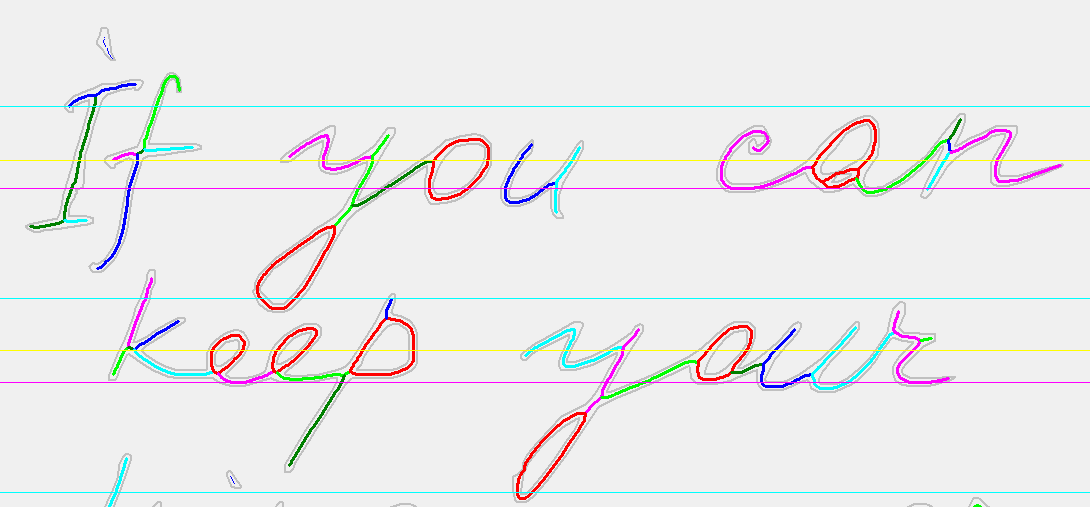
\includegraphics[scale=0.9, height = 5cm]{img/mest9.png}
    	\centering
    	\caption{Результат сегментации}
    	\label{pic:mest1}
    \end{figure}

    Штриховое представление рукописного текста представляет собой структуру данных, в которой каждая запись описывает штрих в виде множества вершин, упорядоченного в соответствии с направлением написания. Каждая вершина задаётся тройкой чисел: её декартовыми координатами и радиусом вписанной окружности, определяющей ширину штриха в этой точке. 

    \begin{figure}[H]
    \begin{minipage}[b]{0.5\textwidth}
        \centering
        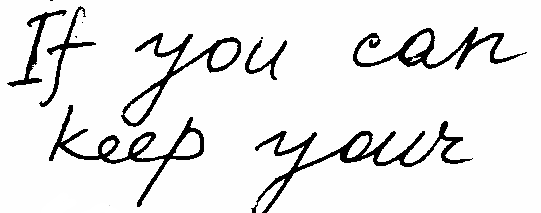
\includegraphics[width=8cm]{img/mest4.png}
        \caption{Бинаризация}
	    \label{pic:14}
    \end{minipage}
     \hfill
    \begin{minipage}[b]{0.5\textwidth}
        \centering
        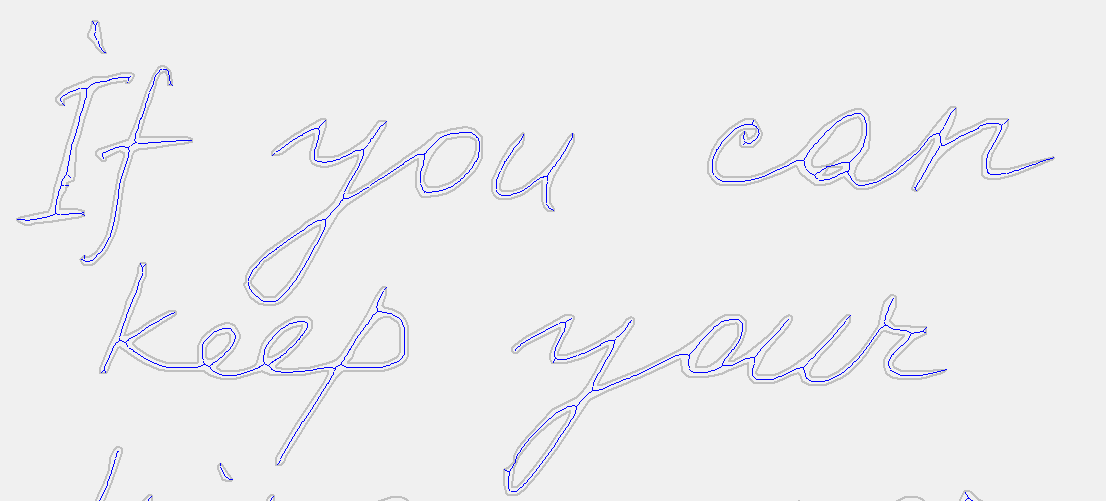
\includegraphics[width=8cm]{img/mest5.png}
        \caption{Аппроксимация и Скелетизация}
	    \label{pic:15}
    \end{minipage}
    \end{figure}
    
    Процесс штриховой сегментации включает в себя несколько шагов: Бинаризацию, Аппроксимацию, Скелетизацию. 
    Изображение текста аппроксимируется многосвязными многоугольными фигурами – многоугольниками с многоугольными дырами. Скелетизация многоугольных фигур состоит в построении срединных осей – множества точек центров вписанных в фигуры окружностей \autoref{pic:15}.

    Сегментация осуществляется на основе скелетного представления растрового изображения в виде геометрического графа. Штрихи формируются в виде подграфов.

    В полученном скелетном графе выделяются подграфы, описывающие штрихи \textit{Кольца} и \textit{Цепи}. 
    Выделение подграфов можно интерпретировать как разрезание геометрического графа по вершинам. Выделение штрихов осуществляется на основе следующих операций: 
    \begin{enumerate} 
        \item Выделение кольцевых циклических штрихов
        \item Разрезание графа по вершинам третьей степени и более высоких степеней
        \item Для полученных штрихов определяется направление и последовательность их прохождения в рукописном тексте
    \end{enumerate}

    % Для этого используется операция \textit{Разрезания тройников} – вершин скелета третьей степени. 

    % Штриховое представление формируется путём последовательного выделения
    % Колец и Цепей в скелетном графе. 

\subsection{Выделение Колец}

    \begin{figure}[H]
    	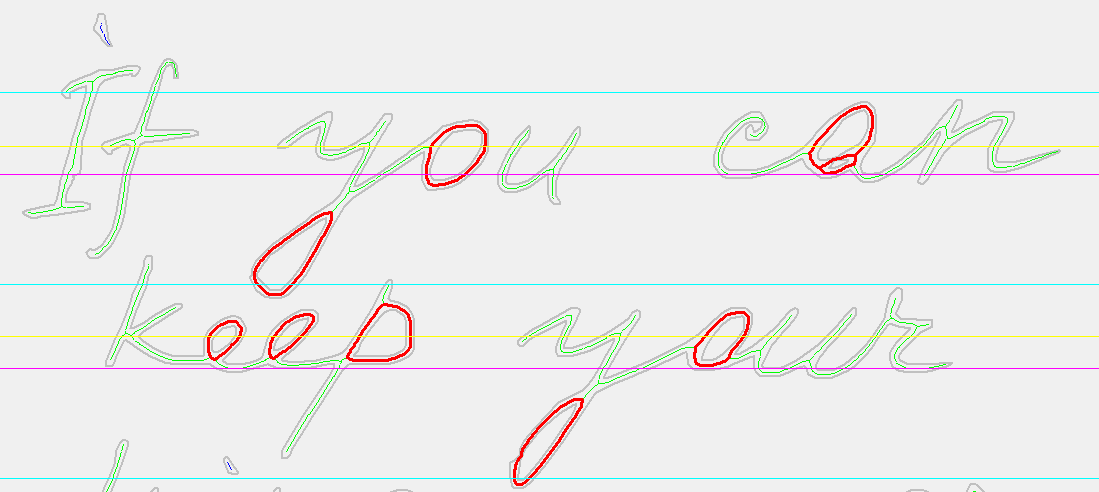
\includegraphics[scale=0.9, height = 5cm]{img/mest6.png}
    	\centering
    	\caption{Выделение кольцевых циклических штрихов}
    	\label{pic:16}
    \end{figure}


    Аппроксимирующие многоугольные фигуры задают подразбиение плоскости изображения на связные компоненты трёх типов: внешняя часть плоскости, внутренние компоненты символов рукописного текста, и компоненты, образующие дыры в многоугольных фигурах. Каждая компонента-дыра определяет кольцевой циклический подграф в скелетном графе. Это даёт возможность выделить все циклические штрихи по следующему правилу. Кольцевые штрихи представляют собой подмножества точек центров вписанных окружностей таких, которые касаются двух разных многоугольников в границах аппроксимирующих многоугольных фигур. 

\subsection{Разрезание тройников}

    В каждой вершине степени 3 строится разрез путём порождения вершины-клона. При этом от основной вершин отделяется одно ребро, в результате чего её степень понижается с 3 до 2. А отрезанное ребро присоединяется к вершине-клону. В результате вновь образованная вершина-клон имеет степень 1 и является терминальной. После разрезания всех вершин третьей степени весь скелетный граф распадается на подграфы Кольца и Цепи.
     
    Для разрезания графа в вершине 3 степени нужно определить, какое из трёх рёбер должно быть отсечено от этой вершины и присоединено к вершине-клону. В том случае, когда тройник входит в какой-либо циклический штрих, отсекается ребро, не входящее в этот штрих. В остальных случаях эта задача решается на основе выбора цепи, имеющей наименьшую кривизну. Вычисляется оценка кривизны цепи, образуемой каждой парой инцидентных узлу рёбер. Для этого выполняется аппроксимация цепи кривой Безье второй степени и вычисляется максимальная кривизна в точках этой гладкой кривой.

    \begin{figure}[H]
    	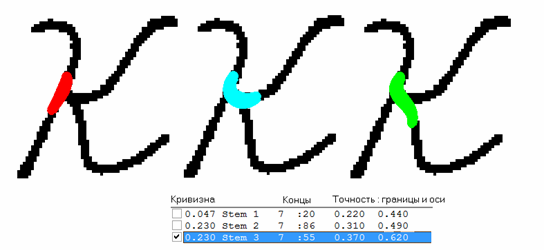
\includegraphics[scale=0.9, height = 5cm]{img/mest7.png}
    	\centering
    	\caption{Разрезание по вершинам третьей степени}
    	\label{pic:17}
    \end{figure}

    Гладкость в большинстве случаев определяет правильно способ разрезания узла третьей степени. Однако в некоторых случаях требуется более тонкий анализ. Для этого может быть использованы правила, построенные на основе машинного обучения.

    Результатом сегментации является полный набор штрихов колец и цепей, образующихся из скелетного графа. 

\subsection{Определение направления и последовательности прохождения штрихов}

    Для определения направления и последовательности прохождения штрихов используется несколько эвристических правил.
    \begin{enumerate} 
        \item Кольцевые штрихи, лежащие в базовой строке и выступающие вверх, нужно обходить против часовой стрелки, а штрихи, свисающие вниз --- по часовой
        \item Штрихи вертикального типа имеют направление сверху вниз, горизонтального типа --- слева направо. Принадлежность к конкретному типу определяется наклоном штриха к горизонтали, например, относительно порога $45^{\circ}$
        \item Цепи, примыкающие к базовым кольцевым штрихам, имеют направление от своей концевой точки, инцидентной кольцевому штриху, ко второй концевой точке
        \item Упорядочение штрихов в базовой строке выполняется естественным образом слева направо по расположению штрихов
        \item Выступающие и свисающие штрихи упорядочиваются непосредственно вслед за базовым штрихом, к которому они примыкают
    \end{enumerate}
\section{Нормализация штрихов}
Важно отметить, что Фурье спектр зависит от расположения ломаной, а также от направления обхода кривой, поэтому важно сначала произвести нормализацию. В данной работе используется следующий подход
\begin{enumerate}
    \item Вычисляется точка, являющаяся центром масс штриха, то есть точка, являющаяся усреднением координат точек штриха.
    \item Осуществляется параллельный перенос штриха так, что центр масс оказывается в начале координат.
    \item Если штрих не является кольцевым, то выставляем порядок обхода так, что начальная точка находится левее конечной. Это преобразование связано с тем, что текст пишется слева направо.
    \item Если штрих является кольцевым, то начинаем обход с самой левой точки штриха по часовой стрелке.
\end{enumerate}
\section{Метрика на основе преобразования Фурье}
После сегментации и нормализации мы имеем представление каждого штриха в виде ломаной $L = \{(x_j, y_j)\}_{j=1}^l$. На нее можно посмотреть, как на последовательность точек в комплексной плоскости $\{x_j + i y_j\}_{j=1}^l$, то есть как на сигнал, для получения векторного представления которого предлагается использовать дискретное преобразование Фурье. 
\par Для первичного определения того, является~ли предлагаемое векторное представление дискриминативным была рассмотрена задача классификации штрихов набора панграмм, изображенного на \autoref{fig:data}.
\begin{figure}[H]
    \centering
    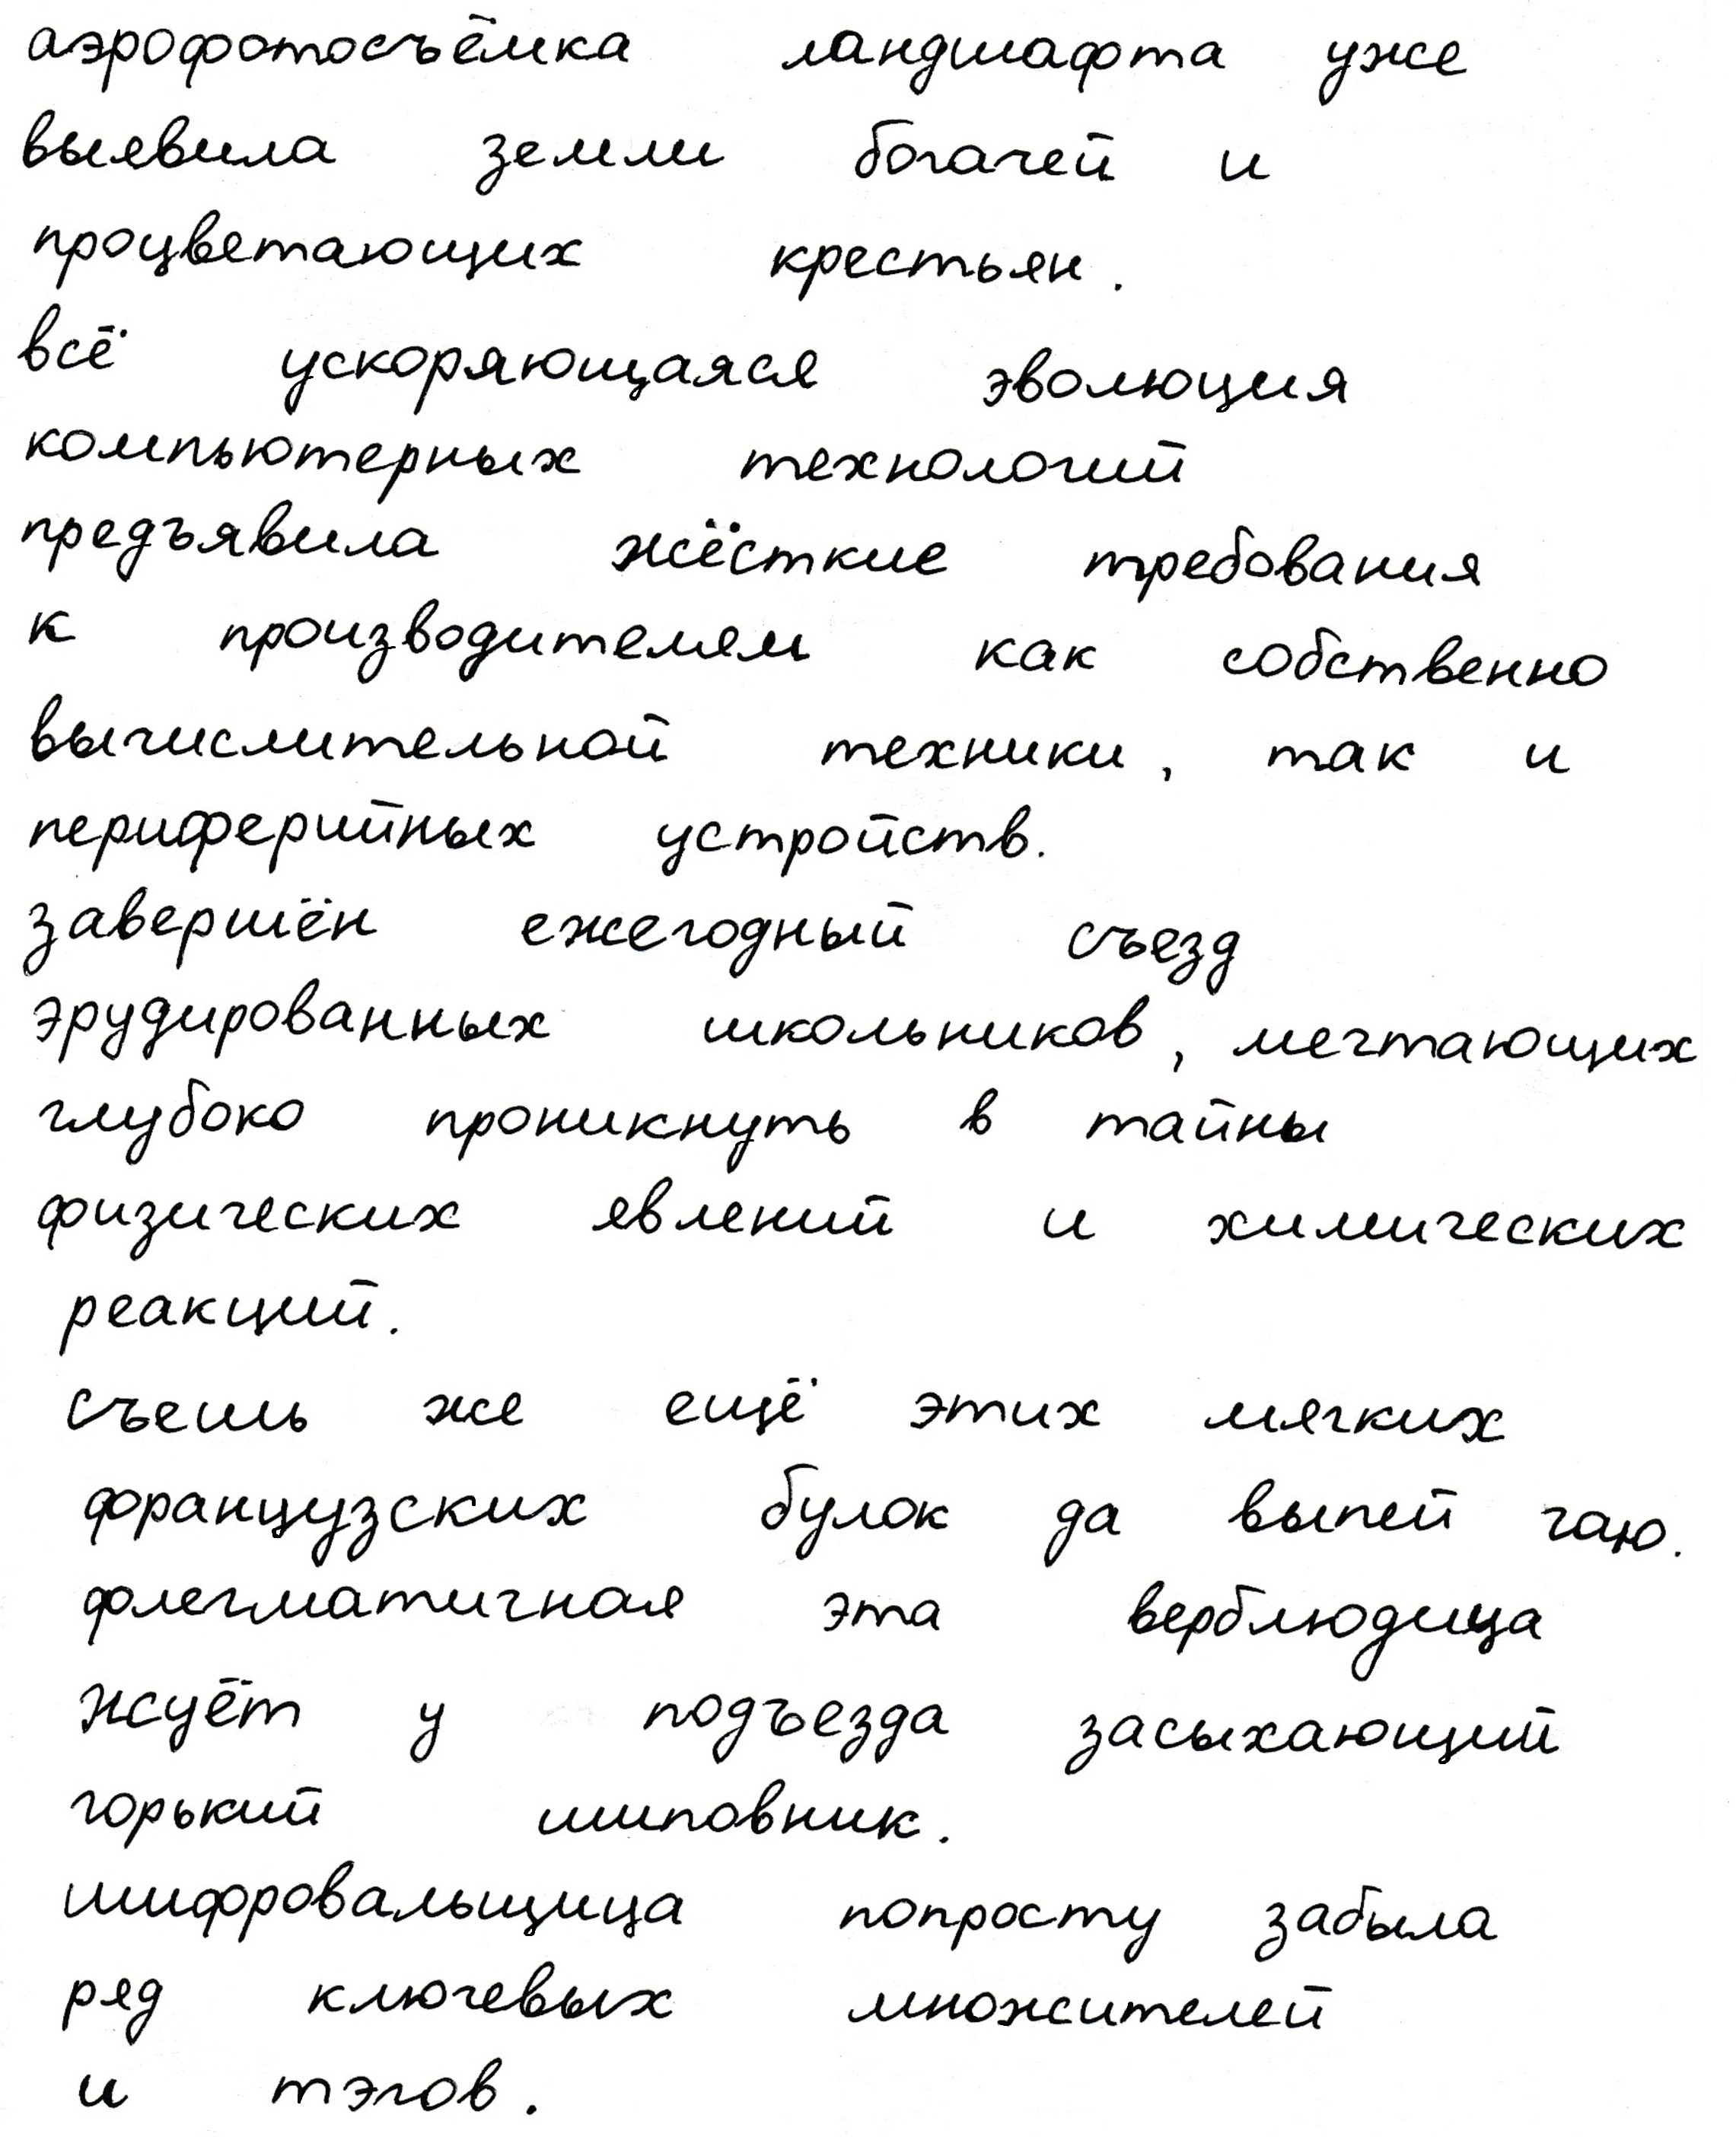
\includegraphics[width=0.3\linewidth]{img/text_my.jpg}
    \caption{Изображение текста, на котором проводились эксперименты}
    \label{fig:data}
\end{figure}

В первую очередь была произведена проверка того, как ведет себя отношение внутриклассового расстояния к межклассовому в евклидовой метрике в зависимости от количества используемых коэффициентов Фурье. 
\par Как видно из \autoref{fig:compactness}, при всех значениях наблюдается выполнение гипотезы компактности, при этом при увеличении количества коэффициентов наблюдается деградация разделимости классов, так как появляются коэффициенты, отвечающие за шумы. 
\par Из этого можно сделать вывод, что для описания штрихов достаточно малого количества коэффициентов Фурье.
\begin{figure}
    \centering
    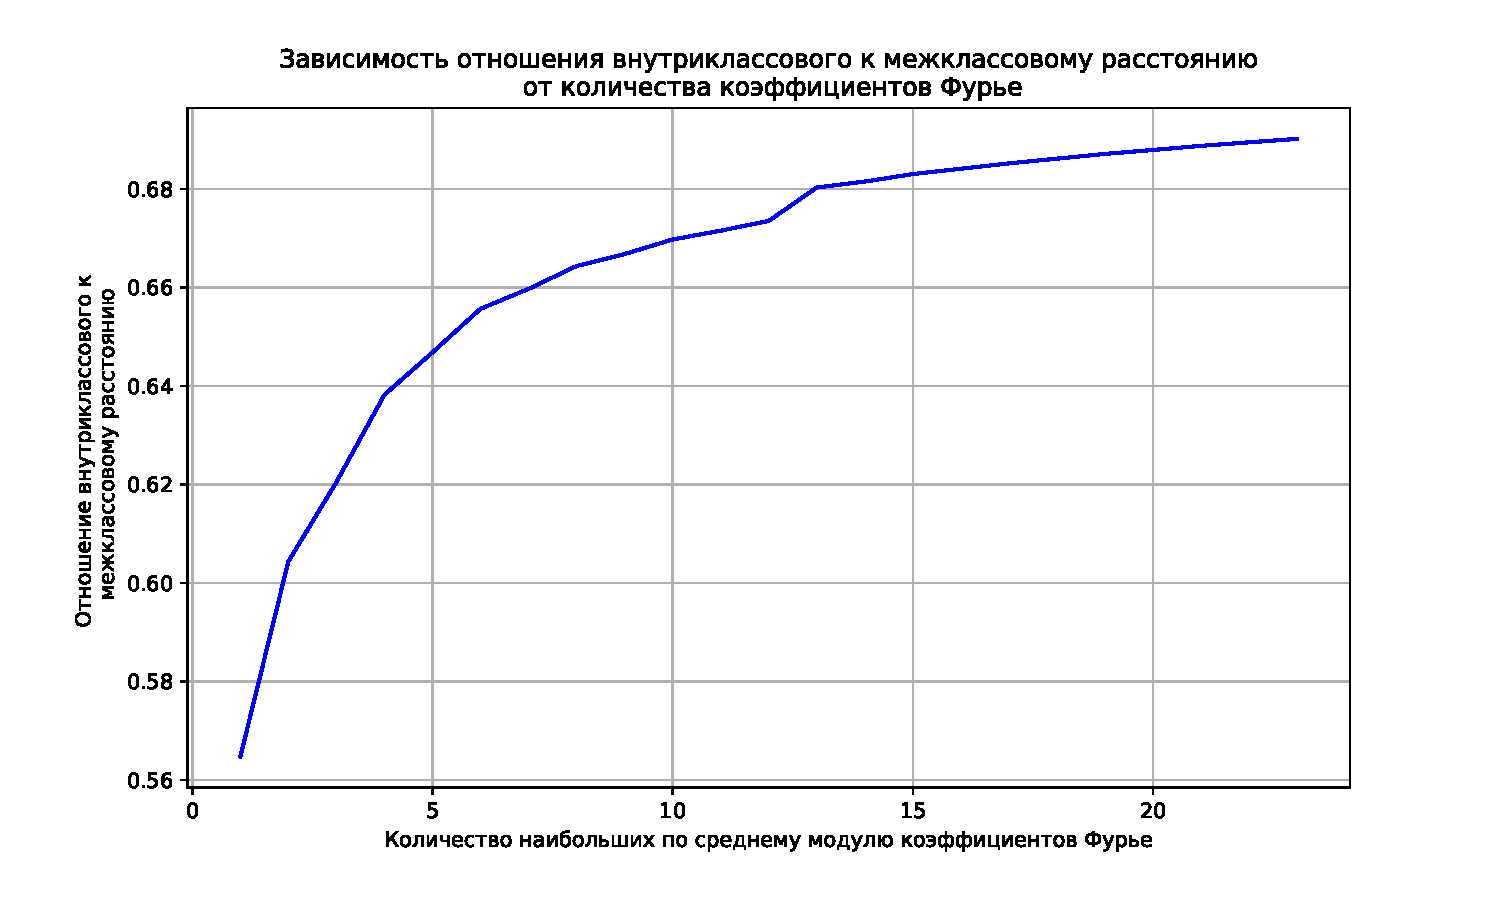
\includegraphics[width=0.49\linewidth]{img/compactness.pdf}
    \caption{Результаты эксперимента, проверяющего гипотезу компактности для различного количества коэффициентов Фурье}
    \label{fig:compactness}
\end{figure}
\par Для проверки предложенной гипотезы решалась задача классификации штрихов методом k ближайших соседей, качество измерялось на кросс валидации с пятью разбиениями выборки с помощью F1-macro метрики, так как она учитывает дисбаланс классов. 
\par Для каждого количества коэффициентов Фурье выбиралось лучшее значение $k$ по результатам кросс валидации, после чего изучались результаты этого алгоритма. 
Как видно из \autoref{fig:classification} существенной разницы между использованием $5$--$23$ коэффициентов Фурье нет: и значение метрики, и ее устойчивость примерно одинаковы. 
Значит, мы можем использовать малое количество признаков, например, $7$ в случае евклидова расстояния и $4$ в случае косинусного. 
\begin{figure}
    \centering
    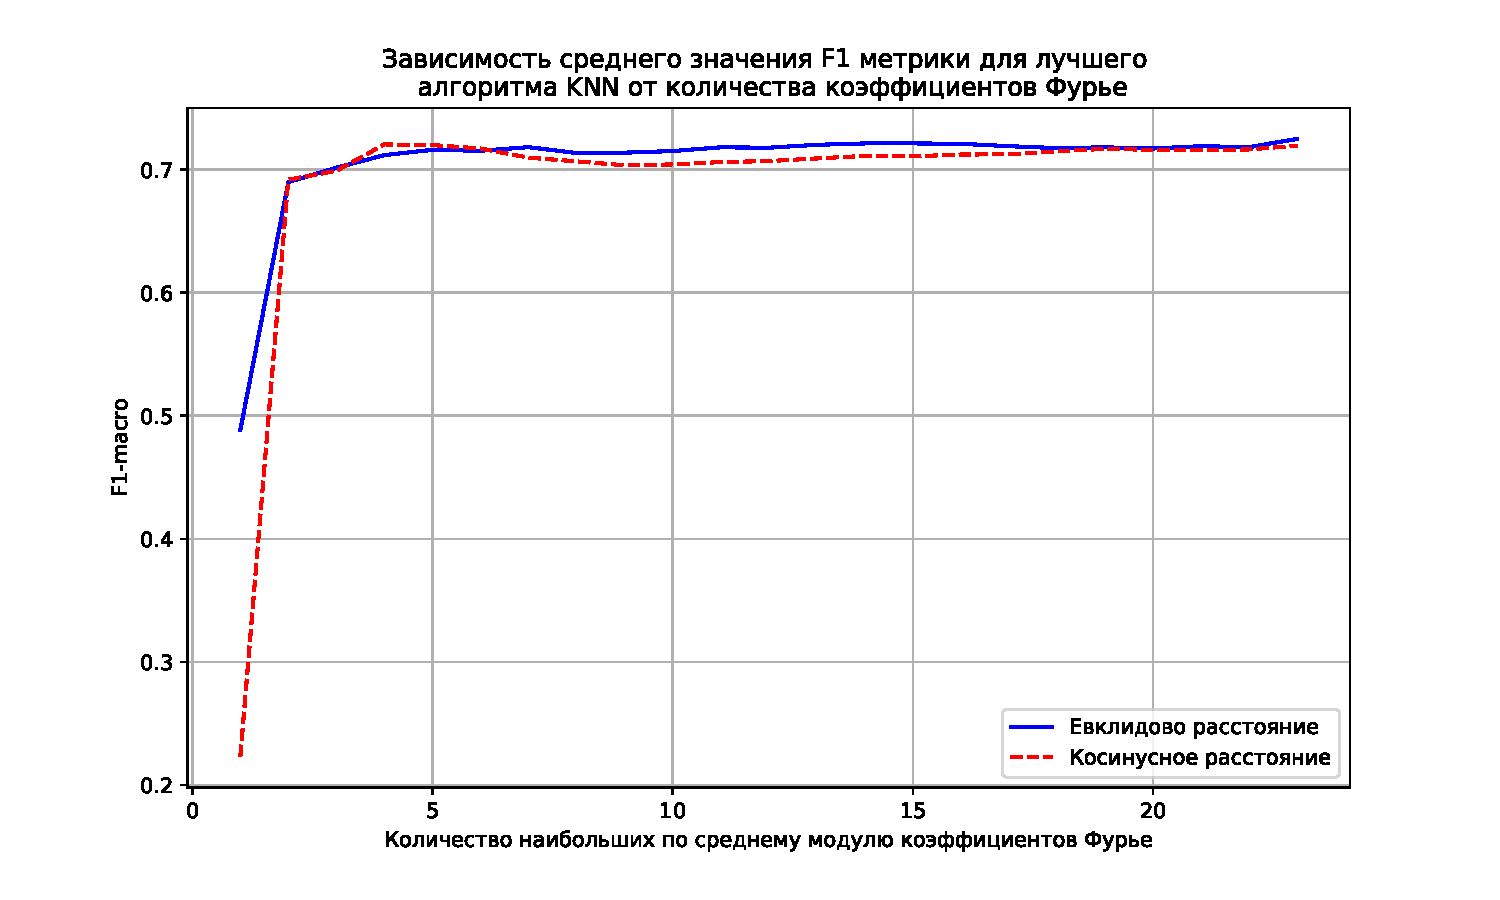
\includegraphics[width=0.49\linewidth]{img/mean.pdf}
    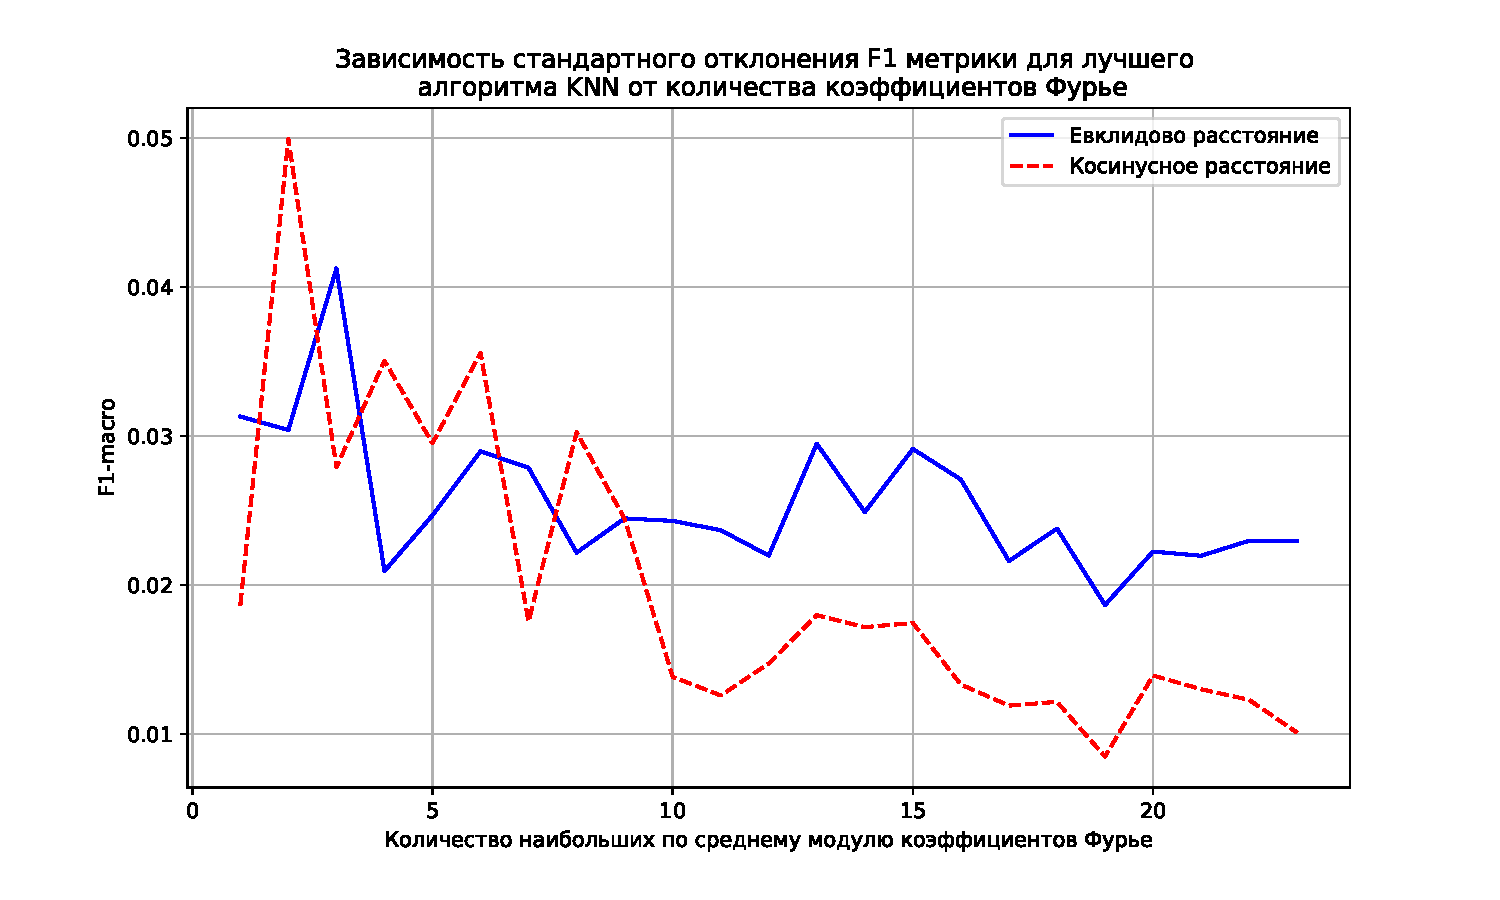
\includegraphics[width=0.49\linewidth]{img/std.pdf}
    \caption{Результаты эксперимента, проверяющего гипотезу компактности для различного количества коэффициентов Фурье}
    \label{fig:classification}
\end{figure}
\section{Сравнение с существующими подходами}
Для сравнения предложенной метрики с существующими предлагается решить задачу классификации штрихов, полученных из изображения \autoref{fig:data}. Всего $1231$ штрих, $12$ классов, каждый из которых соответствует одну типу каллиграфических элементов, в данных наблюдается дисбалланс классов: самый многочисленный класс состоит из $250$ штрихов, самый немногочисленный из $28$. Также в данных есть ошибки в разметке. Размеченные данные изображены на \autoref{fig:classes}.
\begin{figure}[H]
\centering
    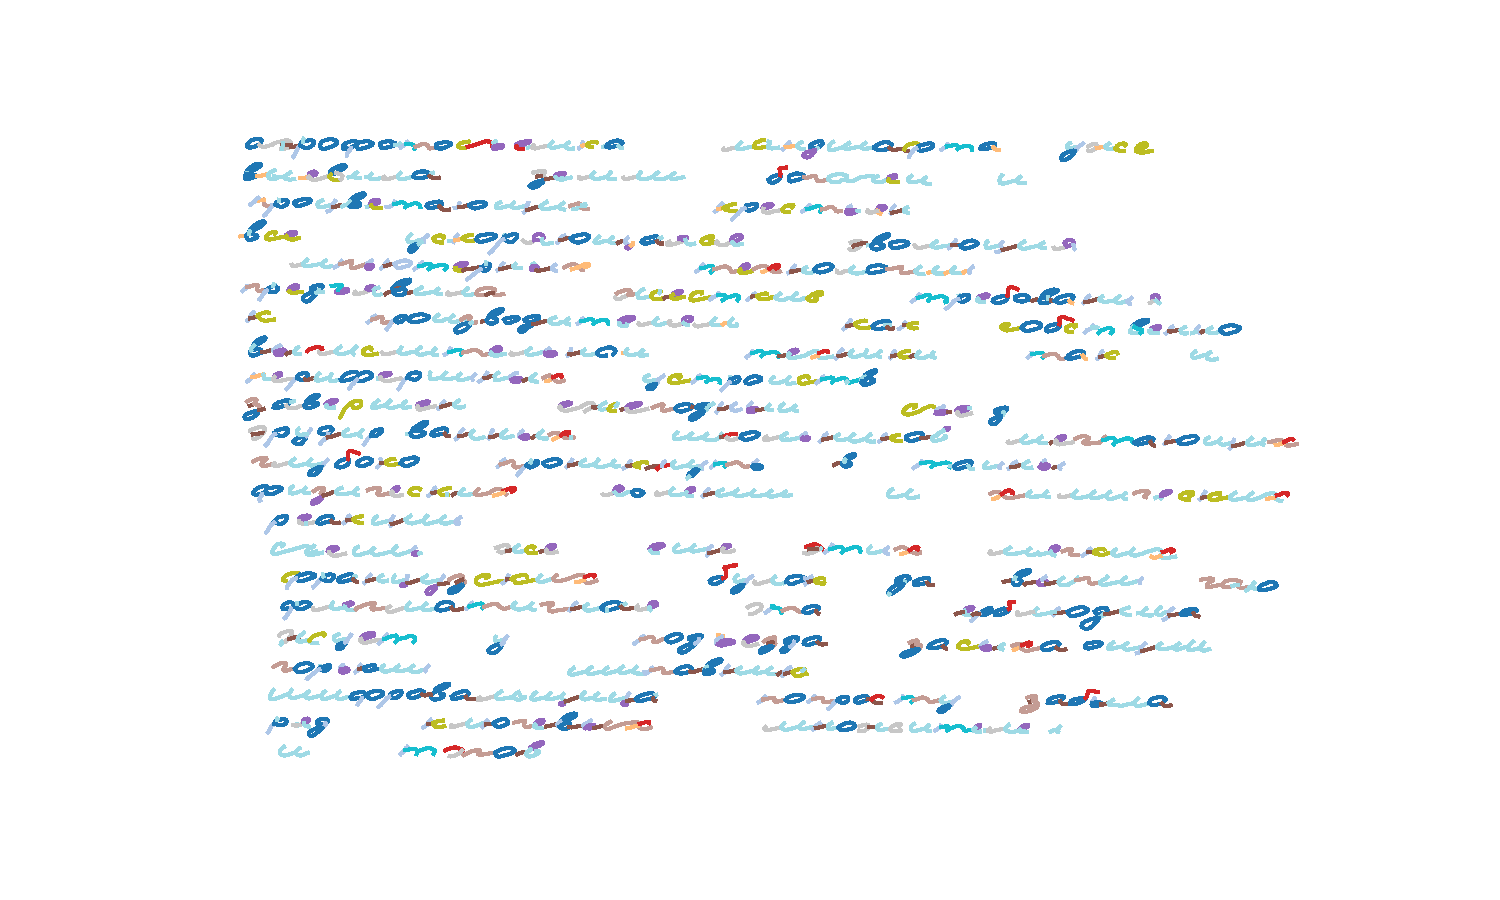
\includegraphics[width=0.8\linewidth, trim={2cm 2cm 2cm 2cm}, clip]{img/classes.pdf}
    \caption{Размеченные данные: каждый цвет соответствует одному классу.}
    \label{fig:classes}
\end{figure}
Будем сравнивать расстояние на основе преобразования Фурье с метриками, предложенными в \citep{pronina2023frechet, pazazia2023dtw}: расстояние Фреше между ломаными, DTW расстояние на коэффициентах сплайнов, аппроксимирующих ломанную, двумерное DTW расстояние между ломаными. Во всех случаях используется предобработка штрихов, которую использовали авторы. Расстояния будем сравнивать с помощью алгоритма KNN, как с равномерными весами, так и с весами, зависящими от расстояния. В качестве метрики качества классификации воспользуемся средним значением F1-macro (так как эта метрика учитывает дисбаланс классов) на кросс-валидации на пяти фолдах. Также изучим устойчивость метрик, изучис стандартное отклонение F1-macro. Результаты эксперимента представлены на \autoref{fig:experiment_mean} и \autoref{fig:experiment_std} соответственно. 

\begin{figure}[H]
\centering
    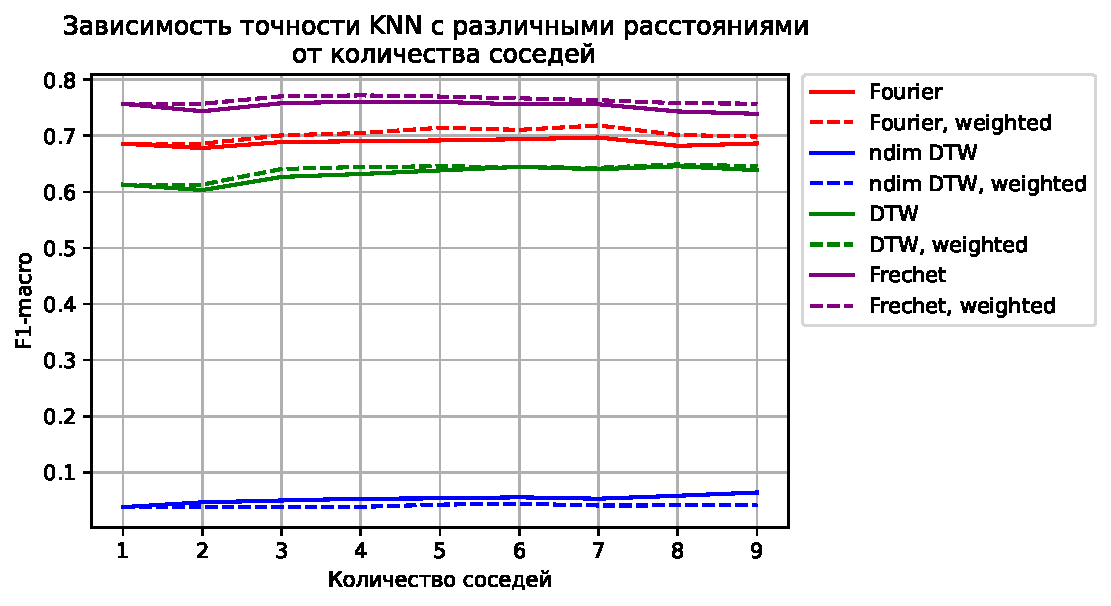
\includegraphics[width=0.6\linewidth]{img/experiment_mean.pdf}
    \caption{Зависимость среднего значения F1-macro на кросс-валидации от количества соседей в алгоритме KNN, красным отмечены значения для расстояния на основе преобразования Фурье, синим отмечены значения для двумерного DTW, фиолетовым для расстояния Фреше, зеленым -- для DTW на коэффициентах сплайнов. Пунктиром отмечены запуски, при которых предсказания зависели от расстояний до соседей, а не только от их классов.}
    \label{fig:experiment_mean}
\end{figure}

\begin{figure}[H]
\centering
    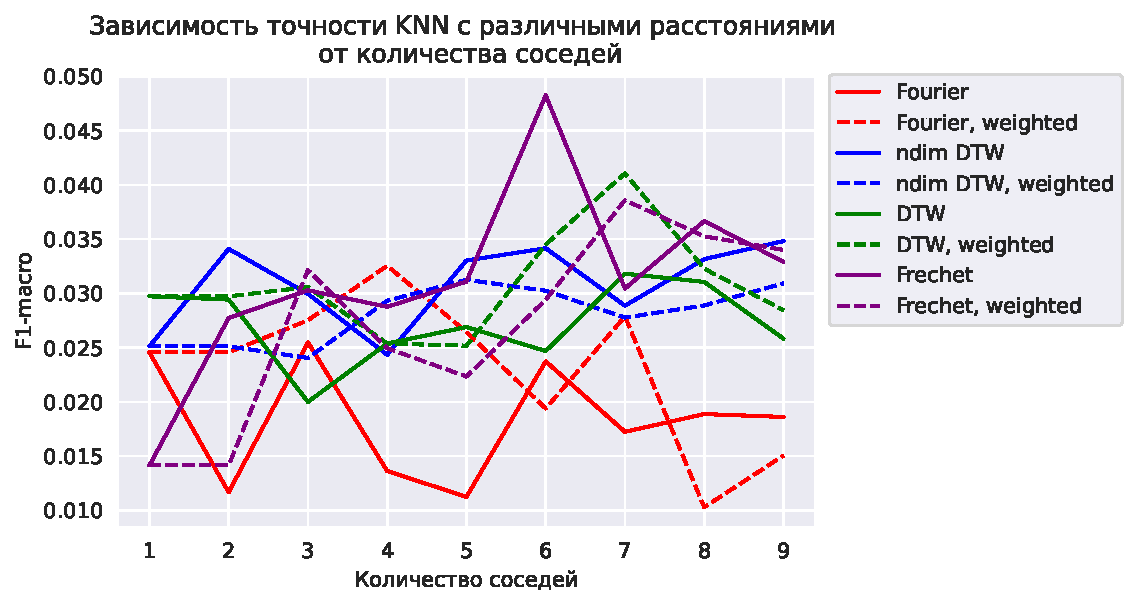
\includegraphics[width=0.6\linewidth]{img/experiment_std.pdf}
    \caption{Зависимость стандартного отклонения F1-macro на кросс-валидации от количества соседей в алгоритме KNN, красным отмечены значения для расстояния на основе преобразования Фурье, синим отмечены значения для двумерного DTW, фиолетовым для расстояния Фреше, зеленым -- для DTW на коэффициентах сплайнов. Пунктиром отмечены запуски, при которых предсказания зависели от расстояний до соседей, а не только от их классов.}
    \label{fig:experiment_std}
\end{figure}

Исходя из графиков, можно сделать несколько выводов:
\begin{enumerate}
    \item Расстояние Фреше дает наибольшую точность.
    \item Расстояние на основе преобразования Фурье идет на втором месте.
    \item Все метрики показывают перфоманс близкий к наилучшему при всех значениях количества соседей. Этот момент важен, так как он говорит о хорошем выполнении гипотезы компактности.
\end{enumerate}

Теперь отметим важное преимущество расстояния на основе преобразования Фурье перед расстоянием Фреше. Вычисление матрицы попарных расстояний между штрихами для рассматриваемого изображения занимает $0.2$ секунды в случае использования предлагаемого расстояния. Расстояние Фреше же требует более $2$-х часов вычислений. Таким образом, с точки зрения использования расстояний для систем поиска расстояние на основе преобразования Фурье является оптимальным среди работ, известных авторам. Также отметим, что полученное векторное представление может быть использовано не только в метрических классификаторах, но и в любых других алгоритмах машинного обучения, что также является преимуществом.
\section{Выводы}
В работе предложено малопараметрическое векторное описание элементов штриховой сегментации на основе преобразования Фурье. Экспериментально показано, что полученные вектора удовлетворяют гипотезе компактности. Также было проведено сравнение предлагаемого расстояния с существующими аналогами, в результате которого было показано, что расстояние на основе преобразования Фурье является лучшим вариантом по соотношению качество/время вычислений. При дальнейшей работе над методом будут изучены возможности другой предобработки, которые сведут использование коэффициентов Фурье только для описания формы, будут добавлены геометрические признаки. Также будет изучена возможность применения данного расстояния для задачи поиска ключевых слов в рукописном контексте, и возможность составления идентификатора почерка на основе средних значений коэффициентов Фурье для штрихов каждого класса.
% Традиционно в данной задаче используются метрики, используемые в информационном поиске. Пусть $w^i_s$ - изображение, стоящее на позиции $i$ в отсортированном по возрастанию значения $f(w, s)$ множестве $W$. Тогда определим метрики качества как:
% $$MAP@K = \frac{1}{|Q|}\sum_{q \in S}\frac{1}{K}\sum_{i=1}^K $$





% \section{Headings: first level}
% \label{sec:headings}

% \lipsum[4] See Section \ref{sec:headings}.

% \subsection{Headings: second level}
% \lipsum[5]
% \begin{equation}
% 	\xi _{ij}(t)=P(x_{t}=i,x_{t+1}=j|y,v,w;\theta)= {\frac {\alpha _{i}(t)a^{w_t}_{ij}\beta _{j}(t+1)b^{v_{t+1}}_{j}(y_{t+1})}{\sum _{i=1}^{N} \sum _{j=1}^{N} \alpha _{i}(t)a^{w_t}_{ij}\beta _{j}(t+1)b^{v_{t+1}}_{j}(y_{t+1})}}
% \end{equation}

% \subsection{Headings: third level}
% \lipsum[6]

% \paragraph{Paragraph}
% \lipsum[7]



% \section{Examples of citations, figures, tables, references}
% \label{sec:others}

% \subsection{Citations}
% Citations use \verb+natbib+. The documentation may be found at
% \begin{center}
% 	\url{http://mirrors.ctan.org/macros/latex/contrib/natbib/natnotes.pdf}
% \end{center}

% Here is an example usage of the two main commands (\verb+citet+ and \verb+citep+): Some people thought a thing \citep{kour2014real, hadash2018estimate} but other people thought something else \citep{kour2014fast}. Many people have speculated that if we knew exactly why \citet{kour2014fast} thought this\dots

% \subsection{Figures}
% \lipsum[10]
% See Figure \ref{fig:fig1}. Here is how you add footnotes. \footnote{Sample of the first footnote.}
% \lipsum[11]

% \begin{figure}
% 	\centering
% 	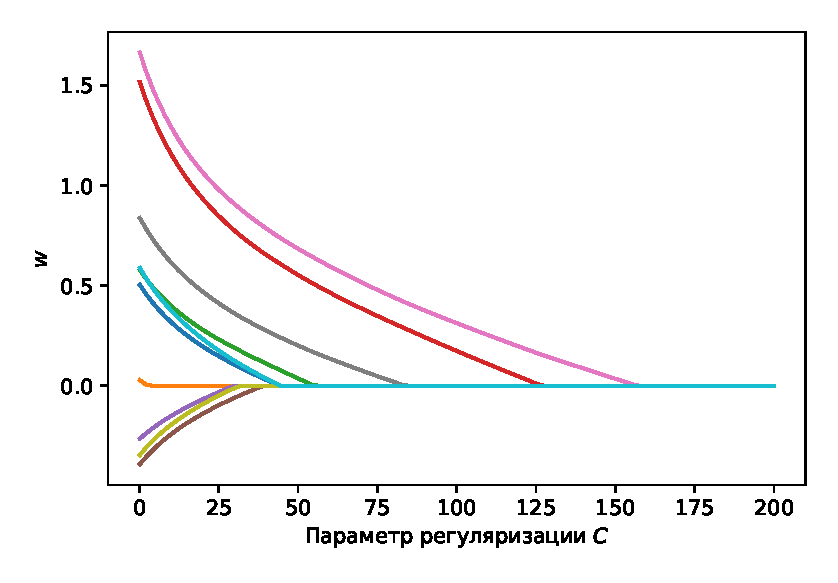
\includegraphics[width=0.5\textwidth]{../figures/log_reg_cs_exp.eps}
% 	\caption{Sample figure caption.}
% 	\label{fig:fig1}
% \end{figure}

% \subsection{Tables}
% See awesome Table~\ref{tab:table}.

% The documentation for \verb+booktabs+ (`Publication quality tables in LaTeX') is available from:
% \begin{center}
% 	\url{https://www.ctan.org/pkg/booktabs}
% \end{center}


% \begin{table}
% 	\caption{Sample table title}
% 	\centering
% 	\begin{tabular}{lll}
% 		\toprule
% 		\multicolumn{2}{c}{Part}                   \\
% 		\cmidrule(r){1-2}
% 		Name     & Description     & Size ($\mu$m) \\
% 		\midrule
% 		Dendrite & Input terminal  & $\sim$100     \\
% 		Axon     & Output terminal & $\sim$10      \\
% 		Soma     & Cell body       & up to $10^6$  \\
% 		\bottomrule
% 	\end{tabular}
% 	\label{tab:table}
% \end{table}

% \subsection{Lists}
% \begin{itemize}
% 	\item Lorem ipsum dolor sit amet
% 	\item consectetur adipiscing elit.
% 	\item Aliquam dignissim blandit est, in dictum tortor gravida eget. In ac rutrum magna.
% \end{itemize}


\bibliographystyle{unsrtnat}
\bibliography{references}

\end{document}